%% ===========================================================================
%%  Latent-space driven active learning of MLIPs for Li|LLZO interfaces
%%  Portrait 84 x 119 cm, DFT-FE theme, two columns, light only.
%%  Layout follows github.com/darakji/oldHiPC2025Poster
%%  Build: tectonic poster_v2.tex
%% ===========================================================================
\documentclass[serif,mathserif,final]{beamer}
\mode<presentation>{\usetheme{DFTFE}}
\usepackage{amsmath,amsfonts,amssymb,pxfonts,eulervm,xspace}
\usepackage{graphicx}
\usepackage{ragged2e}
\usepackage{booktabs}
\usepackage{caption}
\usepackage[many]{tcolorbox}
\usepackage{multirow}
\usepackage{tikz}
\usetikzlibrary{arrows.meta,positioning,shapes,patterns,backgrounds,fit}
\graphicspath{{figs/}{./}}
\usepackage[orientation=portrait,size=custom,height=119,width=84,scale=1.45]{beamerposter}

\newcommand{\DFTFE}{\texttt{DFT-FE}}
\newcommand{\LLZO}{Li$_7$La$_3$Zr$_2$O$_{12}$}

%% -- light palette ---------------------------------------------------------
\definecolor{titlegray}{RGB}{226,234,237}
\definecolor{framegray}{RGB}{150,165,172}
\definecolor{inkblue}{RGB}{23,70,118}
\definecolor{accentred}{RGB}{150,25,35}
\definecolor{goodgreen}{RGB}{20,95,45}
\definecolor{oxide}{RGB}{154,176,201}
\definecolor{metal}{RGB}{206,198,178}
\definecolor{iface}{RGB}{246,214,160}
\definecolor{vac}{RGB}{245,247,248}
\definecolor{dimgraytext}{RGB}{95,100,105}

\tcbset{
  posterbox/.style={
    enhanced, breakable=false,
    colback=white, colframe=framegray,
    colbacktitle=titlegray, coltitle=black,
    fonttitle=\Large\bfseries\scshape,
    boxrule=1.1pt, arc=3mm,
    left=2.5mm, right=2.5mm, top=2mm, bottom=2mm,
    toptitle=1.2mm, bottomtitle=1.2mm,
    titlerule=0pt
  }
}

\newcommand{\good}[1]{\textcolor{goodgreen}{\textbf{#1}}}
\newcommand{\bad}[1]{\textcolor{accentred}{\textbf{#1}}}
\newcommand{\key}[1]{\textcolor{inkblue}{\textbf{#1}}}
\newcommand{\figcap}[1]{\par\vspace{0.25em}{\small\textcolor{dimgraytext}{#1}}}

%% the theme's headline wants logos we do not ship; the header is built in-frame
\setbeamertemplate{headline}{}
\setbeamertemplate{footline}{}
\setbeamertemplate{navigation symbols}{}
\setbeamercolor{postertitle}{fg=black,bg=titlegray}
\setbeamertemplate{itemize item}{\color{inkblue}$\blacksquare$}
\setbeamertemplate{itemize subitem}{\color{framegray}$\blacktriangleright$}

\begin{document}
\setbeamerfont{normal text}{size=\large}
\setbeamerfont{block body}{size=\large}

\begin{frame}[t]

%--- Header ---------------------------------------------------------------
\begin{beamercolorbox}[sep=0.6em,center,wd=\paperwidth]{postertitle}
  {\huge\textbf{Latent-Space Driven Active Learning of Machine-Learned
   Potentials for Solid Electrolyte--Electrode Interfaces}}\\[0.45em]
  {\LARGE\textbf{Application to Li\,$|$\,\LLZO\ at \DFTFE\ Scale}}\\[0.7em]
  {\Large Mehul Darak, \ Rajdeep Boral, \ Kartick Ramakrishnan, \
   Phani Motamarri, \ G.~P.~Das}\\[0.35em]
  {\large Department of Computational and Data Sciences, Indian Institute of
   Science, Bengaluru, India \quad$\bullet$\quad TCG CREST, Kolkata, India}
\end{beamercolorbox}
\vspace{0.35cm}

\begin{columns}[t]

%% =========================== LEFT COLUMN ===============================
\begin{column}{0.48\paperwidth}

\begin{tcolorbox}[posterbox,title=Motivation: the interface decides the battery]
\justifying
Solid-state batteries live or die at the Li-metal\,$|$\,electrolyte interface.
Resolving that chemistry needs molecular dynamics on \textbf{hundreds to
thousands of atoms}, the regime machine-learned interatomic potentials (MLIPs)
were built for.
\vspace{0.3em}
\begin{itemize}
  \item One interface supercell is \textbf{420--1378 atoms}. Orientation,
        termination and Li-site disorder open a configuration space no
        direct-DFT campaign can sample.
  \item Foundation MLIPs are trained overwhelmingly on near-equilibrium
        \emph{bulk}, so interfaces fall outside that distribution and forces
        are \bad{systematically underestimated}.
\end{itemize}
\vspace{0.2em}
\begin{center}\Large
\key{Two questions: what can label these cells at all, and which cells are
worth labelling?}
\end{center}
\end{tcolorbox}

\vspace{0.5em}

\begin{tcolorbox}[posterbox,title=\DFTFE: the engine that makes this possible]
\justifying
\textbf{Every label here is a \DFTFE\ calculation.} \DFTFE\ solves Kohn--Sham
DFT in \textbf{real space} on a finite-element basis: massively parallel,
GPU-accelerated, and the code behind the \key{2023 ACM Gordon Bell Prize}.
\begin{center}
\begin{minipage}[t]{0.485\linewidth}\centering
\vspace{0pt}
{\sffamily\bfseries\small Plane-wave DFT}\\[0.1em]
{\sffamily\footnotesize forced 3D periodicity}\\[0.35em]
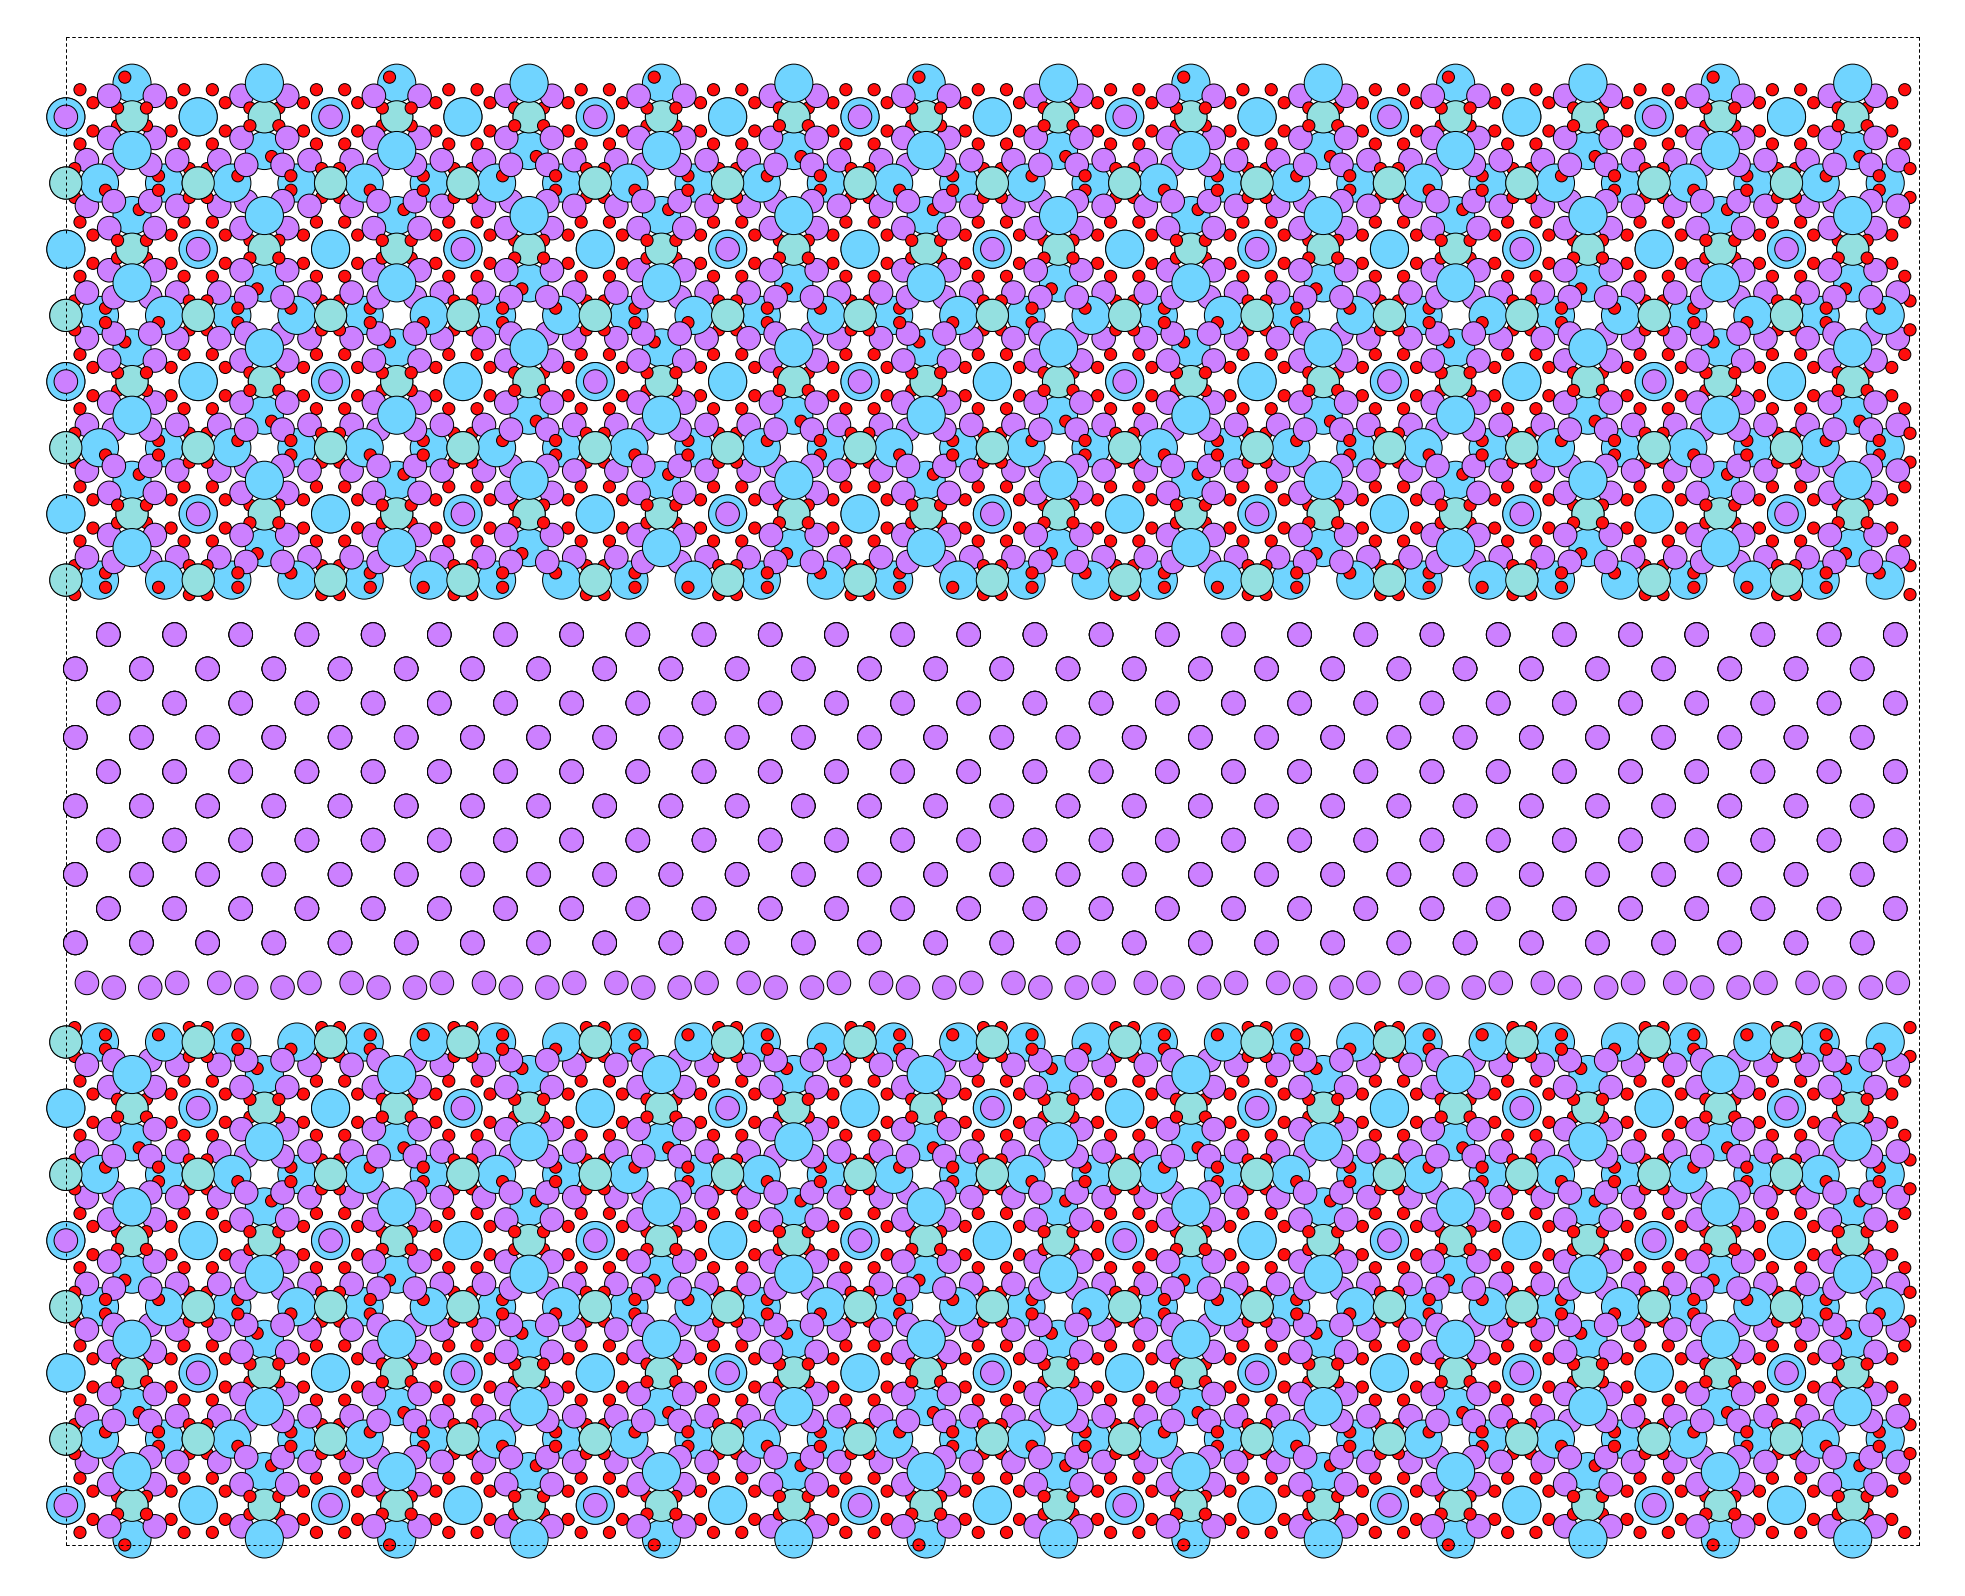
\includegraphics[width=\linewidth]{cell_planewave.png}\\[0.25em]
{\sffamily\footnotesize\color{accentred}two interfaces $\bullet$ image dipole\\no free surface}
\end{minipage}\hfill
\begin{minipage}[t]{0.485\linewidth}\centering
\vspace{0pt}
{\sffamily\bfseries\small \DFTFE}\\[0.1em]
{\sffamily\footnotesize periodic in $x,y$, open in $z$}\\[0.35em]
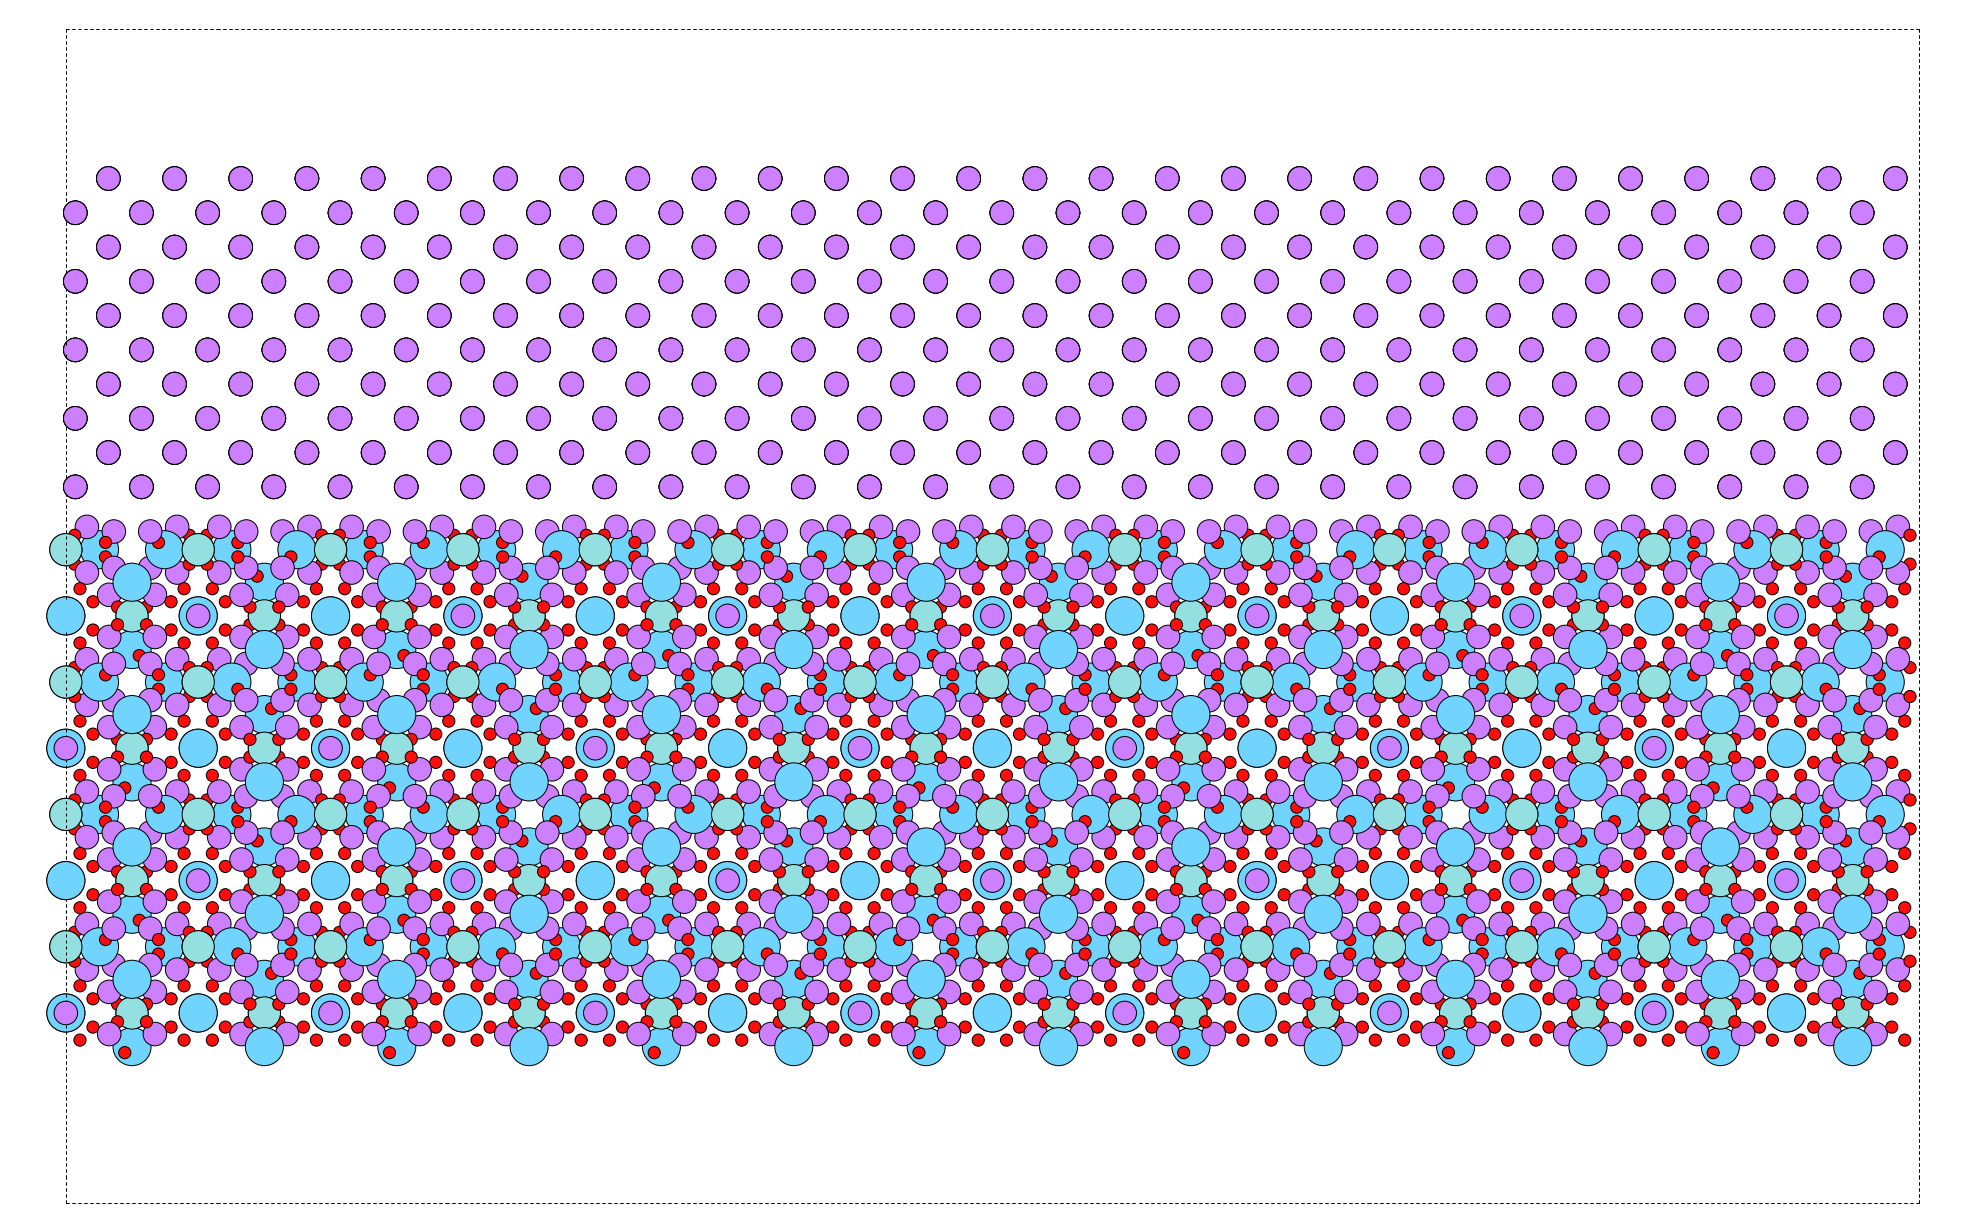
\includegraphics[width=\linewidth]{cell_dftfe.png}\\[0.25em]
{\sffamily\footnotesize\color{goodgreen}one interface $\bullet$ two genuine free surfaces}
\end{minipage}
\end{center}
\figcap{The interface is not a single plane. Chemistry, space charge and the
first liquid-like metal layer occupy a \textbf{band of finite thickness}, which
the open-$z$ cell resolves together with the two free surfaces bounding the
slab.}
\vspace{0.3em}
\begin{itemize}
  \item \key{Semi-periodic boundary conditions.} A finite-element basis is
        local, so periodicity is a choice per direction:
        \texttt{pbc=[True,True,False]}. A plane-wave basis cannot do this;
        3D periodicity forces a \bad{sandwich} with a spurious second
        interface and an image dipole.
  \item \key{Scale.} Real-space domain decomposition puts every label at
        \good{420--1378 atoms}, so the potential is \good{trained at the size
        it is deployed}.
\end{itemize}
\end{tcolorbox}

\vspace{0.5em}

\begin{tcolorbox}[posterbox,title=Coverage-driven active learning]
\justifying
\begin{center}
\begin{tikzpicture}[x=1cm,y=1cm,>=Stealth,
  bx/.style={draw=framegray,very thick,rounded corners=4pt,fill=titlegray,
             text width=7.1cm,minimum height=2.4cm,align=center,
             font=\sffamily\bfseries\footnotesize},
  gx/.style={draw=inkblue,very thick,rounded corners=4pt,fill=oxide!45,
             text width=7.1cm,minimum height=2.4cm,align=center,
             font=\sffamily\bfseries\footnotesize},
  ann/.style={font=\sffamily\tiny,text=dimgraytext,align=center}]
  \node[bx](a) at (0,0)      {Interface\\construction};
  \node[bx](b) at (8.4,0)    {MD sampling\\(NVT)};
  \node[bx](c) at (16.8,0)   {Physicality filter};
  \node[bx](d) at (25.2,0)   {Latent extraction};
  \node[gx](e) at (25.2,-6.0){FPS seeded on\\training set};
  \node[bx](f) at (16.8,-6.0){\DFTFE\ labelling};
  \node[gx](g) at (8.4,-6.0) {LoRA fine-tuning};
  \foreach \i/\j in {a/b,b/c,c/d}{\draw[->,very thick,inkblue](\i)--(\j);}
  \draw[->,very thick,inkblue](d)--(e);
  \draw[->,very thick,inkblue](e)--(f);
  \draw[->,very thick,inkblue](f)--(g);
  \draw[->,very thick,dashed,accentred](g)--(b);
  \node[ann] at (25.2,-8.1){coverage-driven};
  \node[ann] at (16.8,-8.1){420--1378 atoms, open $z$};
  \node[ann] at (8.4,-8.1) {rank 5, $<$1\% of parameters};
  \node[font=\sffamily\bfseries\small,text=inkblue] at (12.6,2.4)
    {seven rounds, it0 $\rightarrow$ it6};
  \begin{scope}[on background layer]
    \draw[dashed,very thick,framegray,rounded corners=6pt]
      (-3.4,1.7) rectangle (28.6,-8.9);
  \end{scope}
\end{tikzpicture}
\end{center}
\vspace{0.3em}
Candidates are embedded with the \textbf{current} model: the rotationally
invariant ($\ell=0$) scalars of the final interaction block, mean-pooled to one
vector $\mathbf{Z}_S$ per structure. Distance there is the model's own measure
of chemical difference, and pretrained representations have been shown to be
strong acquisition signals for active learning of MLIPs [4].
\vspace{0.2em}
\end{tcolorbox}

\end{column}

%% =========================== RIGHT COLUMN ==============================
\begin{column}{0.48\paperwidth}

\begin{tcolorbox}[posterbox,title=Accuracy against \DFTFE]
\justifying
\begin{minipage}[t]{0.56\linewidth}
\vspace{0pt}
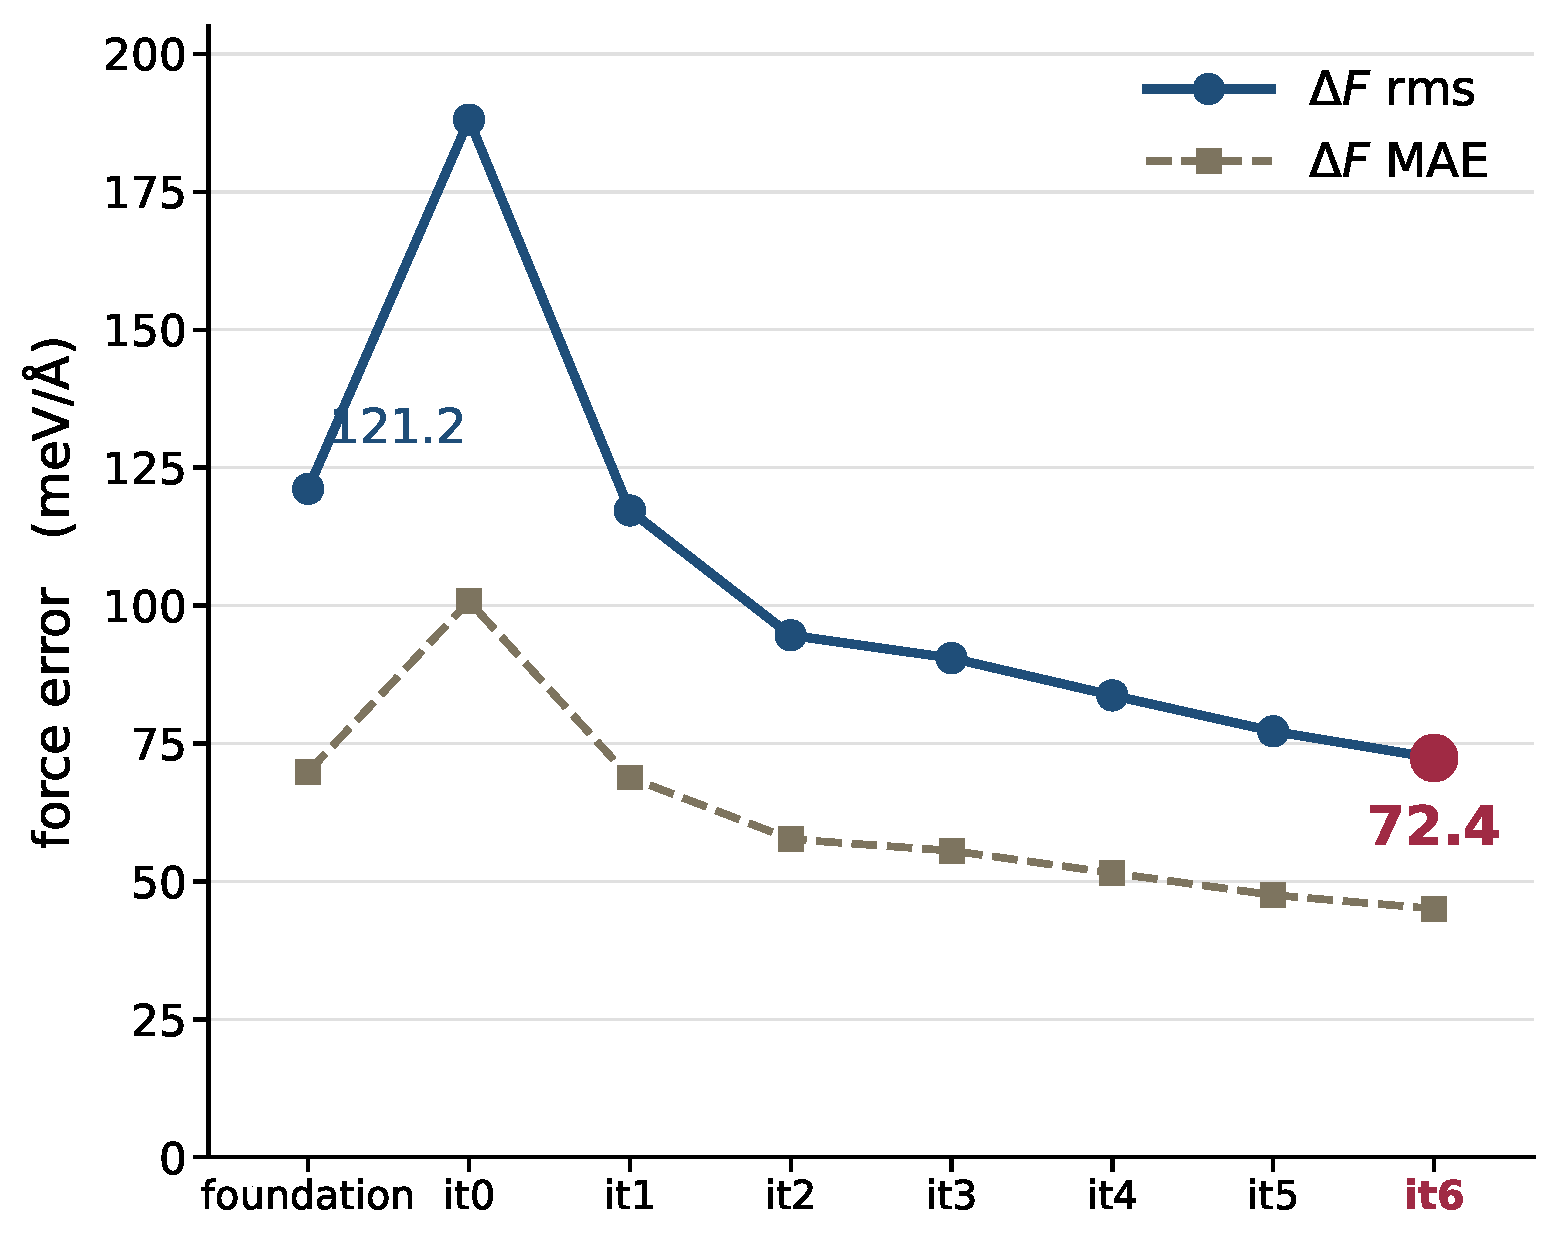
\includegraphics[width=\linewidth]{fig_error_big.pdf}
\end{minipage}\hfill
\begin{minipage}[t]{0.41\linewidth}
\vspace{0pt}
\centering\normalsize
\begin{tabular}{lrrr}
\toprule
\textbf{model} & $\Delta E$ & \multicolumn{2}{c}{$\Delta F$}\\
\cmidrule(lr){2-2}\cmidrule(lr){3-4}
 & meV/at. & rms & MAE\\
\midrule
foundation & \bad{16.0} & \bad{121.2} & \bad{69.9}\\
it0        & 8.3 & 188.1 & 100.8\\
it1        & 5.1 & 117.2 &  68.8\\
it2        & 3.5 &  94.6 &  57.7\\
it3        & 4.6 &  90.5 &  55.6\\
it4        & 3.9 &  83.7 &  51.5\\
it5        & 3.8 &  77.2 &  47.5\\
\midrule
\textbf{it6} & \good{4.1} & \good{72.4} & \good{45.1}\\
\bottomrule
\end{tabular}
\end{minipage}
\figcap{Force error across the campaign on a carefully chosen 33-structure
held-out test set. Forces in meV/\AA. Every round improves on the one before
it.}
\vspace{0.3em}
\begin{itemize}
  \item \good{$-$40\% force rms} and \good{$-$35\% MAE} against the foundation
        model, improving monotonically across the campaign.
  \item \good{$4\times$ lower energy error}: cohesive-energy error falls from
        \bad{16\,meV/atom} on the foundation model to \good{$\sim$4\,meV/atom},
        reached early and held through every later round.
\end{itemize}
{\small Held-out structures are independent \DFTFE\ single-point calculations.
The foundation-model energy is a cohesive-energy error referenced to VASP, the
only form in which the two conventions are comparable.}
\end{tcolorbox}

\vspace{0.5em}

\begin{tcolorbox}[posterbox,title=Data efficiency across the campaign]
\justifying
\begin{center}\large
\begin{tabular}{lr}
\toprule
configurations screened (five recorded rounds) & 414{,}019 \\
\textbf{\DFTFE\ labelled, total}               & \key{108} \\
local environments learned from                & \good{73{,}634} \\
held-out test structures                       & 33 \\
cell size, atoms                               & 420--1378 \\
\bottomrule
\end{tabular}
\end{center}
\vspace{0.3em}
MACE sees each atom inside its cutoff sphere, so \textbf{every atom in a
labelled cell is a training example}: 108 structures buy 73{,}634 local
environments, a \good{680$\times$} multiplier on the \DFTFE\ budget.
\end{tcolorbox}

\vspace{0.5em}

\begin{tcolorbox}[posterbox,title=Conclusions,colframe=inkblue]
\justifying
\begin{itemize}
  \item \key{\DFTFE\ is the enabler.} Semi-periodic boundary conditions,
        impossible in a plane-wave basis, plus ground states on
        420--1378-atom cells.
  \item \key{Coverage-driven latent selection} spends a fixed budget on the
        configurations farthest from everything already labelled, and provably
        never re-labels a near-duplicate.
  \item \key{Force error cut 40\%, energy error cut $4\times$} against the
        foundation model, with \key{LoRA} ($r=5$, $<$1\% of parameters)
        leaving the pretrained bulk chemistry intact.
\end{itemize}
\end{tcolorbox}

\vspace{0.5em}

\begin{beamercolorbox}[wd=\linewidth,leftskip=1em]{references}
{\small\textbf{References:}\ [1] Batatia \emph{et al.}, \emph{NeurIPS}
\textbf{35}, 11423 (2022).\ \ [2] Motamarri \emph{et al.}, \emph{CPC}
\textbf{246}, 106853 (2020).\ \ [3] Hu \emph{et al.}, \emph{ICLR} (2022).\ \
[4] Varga-Umbrich \emph{et al.}, \emph{ICML} (2026), arXiv:2605.03964.
\quad\textbf{Acknowledgements:} MATRIX Lab, IISc Bengaluru; OLCF Frontier;
PARAM Rudra.}
\end{beamercolorbox}

\vspace{0.5em}

\begin{tcolorbox}[posterbox,title=Coverage: how a round is chosen and stopped]
\justifying
\begin{equation*}
k^{*}=\operatorname*{arg\,max}_{k\in\mathcal{P}}\,
\min_{s\in\mathcal{S}}\lVert \mathbf{Z}_k-\mathbf{Z}_s\rVert_2,
\quad
\delta_k=\min_{s\in\mathcal{S}}\lVert \mathbf{Z}_k-\mathbf{Z}_s\rVert_2,
\quad \rho=\max_k \delta_k
\end{equation*}
\begin{minipage}[t]{0.53\linewidth}
\vspace{0pt}
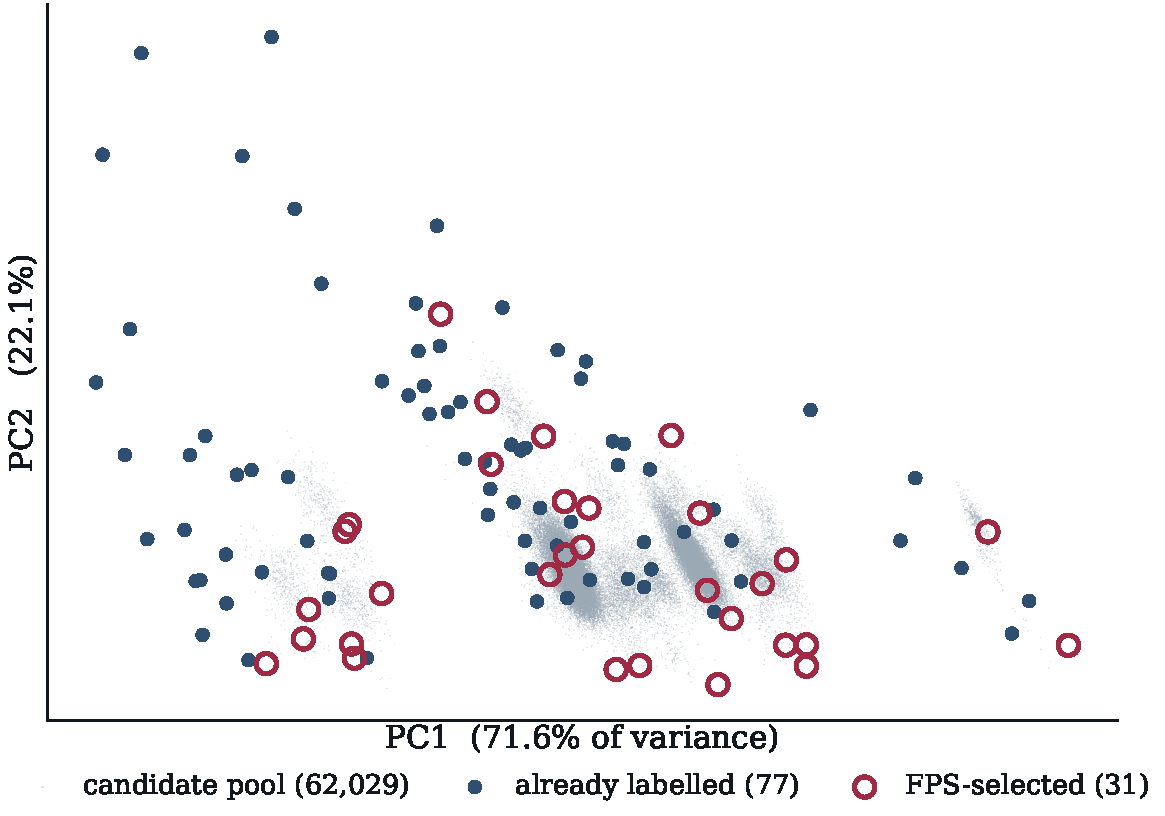
\includegraphics[width=\linewidth]{fig_latent.pdf}
\end{minipage}\hfill
\begin{minipage}[t]{0.44\linewidth}
\vspace{0pt}
Seeding on the set already labelled means a near-duplicate \good{can never be
selected}, so de-duplication is guaranteed by construction.
\vspace{0.3em}

A round closes when the worst-covered candidate falls inside the chosen
percentile of $C(d)=|\{k:\delta_k\le d\}|/|\mathcal{P}|$, so there is no
guesswork about when to stop.
\end{minipage}
\figcap{First two principal components of the mean-pooled latents, one round
shown as illustration. The seed fills the dense core; every new pick lands on
the sparse rim.}
\end{tcolorbox}

\end{column}
\end{columns}
\end{frame}
\end{document}
